\documentclass[aspectratio=169,11pt]{beamer}

\usepackage[T1]{fontenc}
\usepackage{lmodern}
\usepackage{xcolor}
\usepackage{tikz}
\usetikzlibrary{positioning,arrows.meta,calc,fit,shapes.geometric,backgrounds,decorations.pathreplacing,decorations.markings}
\usepackage{booktabs}
\usepackage{array}
\usepackage{graphicx}

\usetheme{default}
\usecolortheme{seahorse}
\setbeamertemplate{navigation symbols}{}
\setbeamertemplate{footline}[frame number]
\setbeamerfont{frametitle}{size=\Large,series=\bfseries}
\setbeamercolor{frametitle}{fg=black}
\setbeamercolor{title}{fg=black}
\setbeamercolor{normal text}{fg=black}

% Custom TikZ styles ---------------------------------------------------------
\tikzset{
  blk/.style    ={draw, rectangle, rounded corners=2pt, align=center, fill=blue!6, minimum height=1.0cm, minimum width=2.4cm, font=\small},
  bigblk/.style ={draw, rectangle, rounded corners=2pt, align=center, fill=blue!6, minimum height=2.2cm, minimum width=4.2cm, font=\small},
  mem/.style    ={draw, rectangle, align=center, fill=orange!12, minimum height=0.7cm, minimum width=3.0cm, font=\small},
  bus/.style    ={draw, rectangle, align=center, fill=orange!16, minimum height=0.8cm, minimum width=8cm, rounded corners=2pt, font=\small},
  io/.style     ={draw, ellipse, align=center, fill=gray!15, minimum height=1.2cm, minimum width=2.6cm, font=\small},
  fsm/.style    ={draw, circle, fill=blue!8, minimum size=1.4cm, font=\small, align=center, inner sep=1pt},
  pipe/.style   ={draw, rectangle, fill=blue!8, minimum width=2.5cm, minimum height=1.4cm, align=center, rounded corners=1pt, font=\small},
  latch/.style  ={draw, rectangle, fill=orange!18, minimum width=0.5cm, minimum height=1.4cm, font=\small},
  arr/.style    ={-{Latex[length=2.5mm]}, thick},
  arrow/.style  ={-{Latex[length=2.5mm]}, thick},
}

\title{No Man's Land}
\subtitle{A custom SystemVerilog GPU and game on the DE1-SoC}
\author{Rohit Biswas \and Kambinachi Obioha \and Nicola Paparella}
\institute{CSEE 4840 --- Embedded System Design --- Spring 2026}
\date{}

\begin{document}

% ===========================================================================
\begin{frame}[plain]
  \titlepage
  \vfill
  \begin{center}
    \small Instructor: Prof.\ Stephen Edwards
  \end{center}
\end{frame}

% ===========================================================================
\begin{frame}[plain]{The system, running}
\centering
\IfFileExists{../submission/img/01_system_running.jpg}{%
  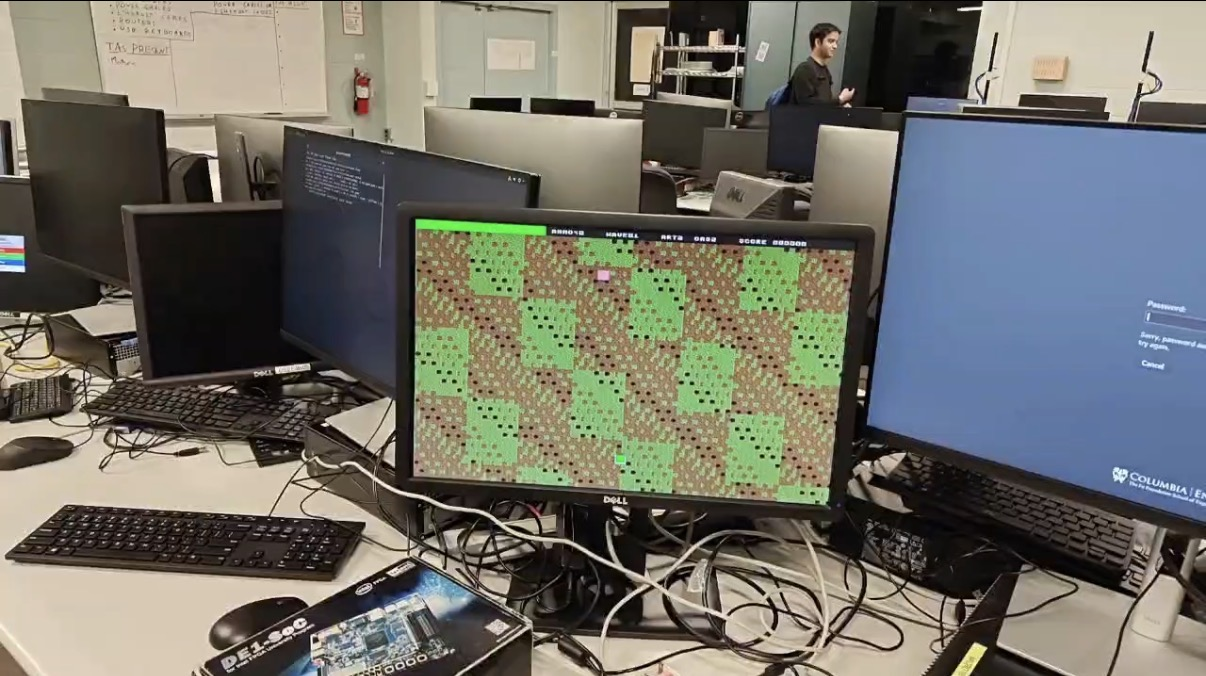
\includegraphics[width=\textwidth,height=0.85\textheight,keepaspectratio]{../submission/img/01_system_running.jpg}%
}{%
  \begin{tikzpicture}
    \draw[thick,dashed,gray] (0,0) rectangle (15,7.5);
    \node at (7.5,4.2) {\Large PHOTO GOES HERE};
    \node at (7.5,3.5) {\small \texttt{submission/img/01\_system\_running.jpg}};
    \node at (7.5,2.8) {\small Board $\bullet$ VGA monitor $\bullet$ SNES gamepad, running};
  \end{tikzpicture}%
}
\end{frame}

% ===========================================================================
\begin{frame}{System block}
\centering
\resizebox{0.95\textwidth}{!}{%
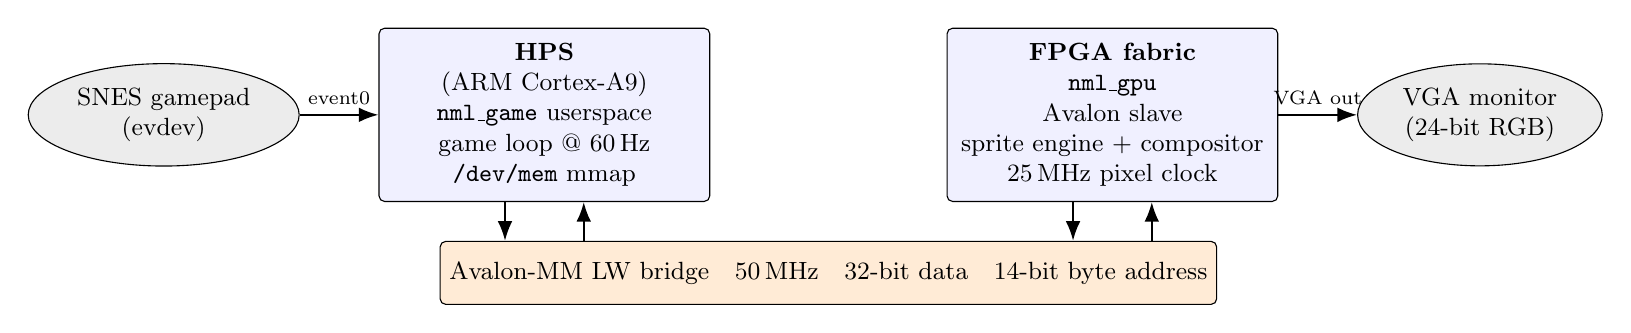
\begin{tikzpicture}[font=\small]
  \node[bigblk] (hps)  {\textbf{HPS}\\(ARM Cortex-A9)\\\texttt{nml\_game} userspace\\game loop @ 60\,Hz\\\texttt{/dev/mem} mmap};
  \node[bigblk, right=3cm of hps] (fpga) {\textbf{FPGA fabric}\\\texttt{nml\_gpu}\\Avalon slave\\sprite engine + compositor\\25\,MHz pixel clock};
  \node[io, left=1cm of hps]   (pad) {SNES gamepad\\(evdev)};
  \node[io, right=1cm of fpga] (vga) {VGA monitor\\(24-bit RGB)};
  \node[bus, below=1.6cm of $(hps)!0.5!(fpga)$] (bus) {Avalon-MM LW bridge\quad 50\,MHz\quad 32-bit data\quad 14-bit byte address};

  \draw[arr] ([xshift=-5mm]hps.south)  -- ([xshift=-5mm]hps.south  |- bus.north);
  \draw[arr] ([xshift= 5mm]hps.south  |- bus.north) -- ([xshift= 5mm]hps.south);
  \draw[arr] ([xshift=-5mm]fpga.south) -- ([xshift=-5mm]fpga.south |- bus.north);
  \draw[arr] ([xshift= 5mm]fpga.south |- bus.north) -- ([xshift= 5mm]fpga.south);
  \draw[arr] (pad.east) -- (hps.west) node[midway, above]{\scriptsize event0};
  \draw[arr] (fpga.east) -- (vga.west) node[midway, above]{\scriptsize VGA out};
\end{tikzpicture}}

\vspace{0.4cm}
\small HPS writes shadow state; FPGA latches at VSYNC; pixels always stream.
\end{frame}

% ===========================================================================
\begin{frame}{What's inside \texttt{nml\_gpu}}
\centering
\resizebox{0.95\textwidth}{!}{%
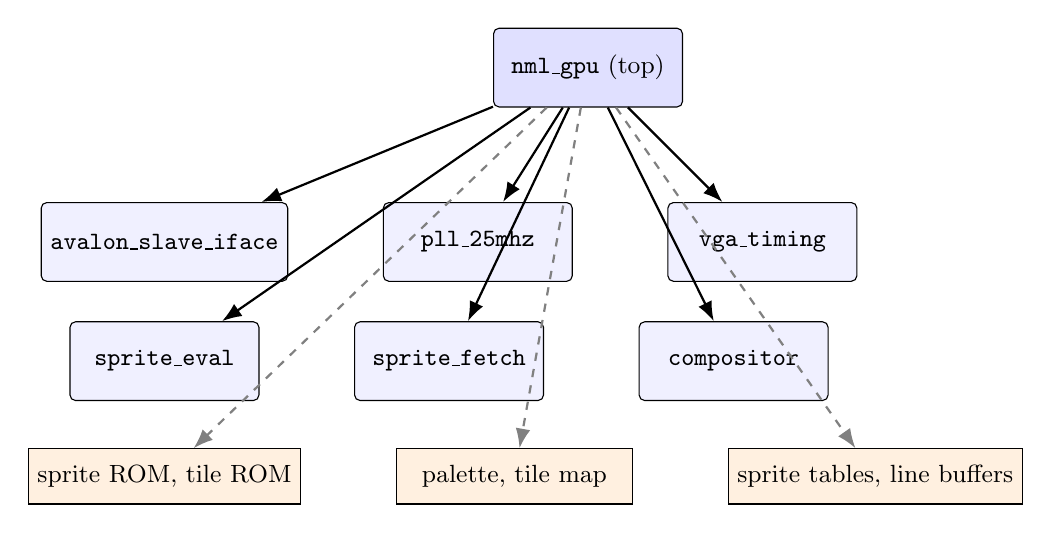
\begin{tikzpicture}[font=\small, node distance=0.5cm and 1.2cm]
  \node[blk, fill=blue!12] (top) {\texttt{nml\_gpu} (top)};
  \node[blk, below left=1.2cm and 2.6cm of top]   (av) {\texttt{avalon\_slave\_iface}};
  \node[blk, right=of av] (pll) {\texttt{pll\_25mhz}};
  \node[blk, right=of pll] (vt) {\texttt{vga\_timing}};
  \node[blk, below=of av]  (se) {\texttt{sprite\_eval}};
  \node[blk, right=of se]  (sf) {\texttt{sprite\_fetch}};
  \node[blk, right=of sf]  (cp) {\texttt{compositor}};

  \node[mem, below=0.6cm of se] (m1) {sprite ROM, tile ROM};
  \node[mem, right=of m1] (m2) {palette, tile map};
  \node[mem, right=of m2] (m3) {sprite tables, line buffers};

  \draw[arr] (top) -- (av);   \draw[arr] (top) -- (pll);  \draw[arr] (top) -- (vt);
  \draw[arr] (top) -- (se);   \draw[arr] (top) -- (sf);   \draw[arr] (top) -- (cp);
  \draw[arr,dashed,gray] (top) -- (m1); \draw[arr,dashed,gray] (top) -- (m2); \draw[arr,dashed,gray] (top) -- (m3);
\end{tikzpicture}}

\vspace{0.3cm}
\small One 50\,MHz domain (Avalon) + one 25\,MHz domain (pixel). All RAMs/ROMs inferred as M10K.
\end{frame}

% ===========================================================================
\begin{frame}{Avalon register map --- 16\,KB window at 0xFF200000}
\centering
\small
\renewcommand{\arraystretch}{1.15}
\begin{tabular}{lll}
\toprule
\textbf{Offset} & \textbf{Name} & \textbf{Layout} \\
\midrule
\texttt{0x0000} & \texttt{CTRL}         & \texttt{[0]}=ENABLE, \texttt{[1]}=SWAP (auto-clear), \texttt{[2]}=HUD\_ON \\
\texttt{0x0004} & \texttt{STATUS}       & \texttt{[0]}=VBLANK, \texttt{[1]}=SWAP\_PENDING \\
\texttt{0x0008} & \texttt{BG\_SCROLL}   & \texttt{[15:0]}=scroll\_x, \texttt{[31:16]}=scroll\_y (signed) \\
\texttt{0x000C} & \texttt{IRQ\_MASK}    & \texttt{[0]}=VBLANK IRQ enable \\
\texttt{0x0010} & \texttt{PLAYER\_POS}  & \texttt{[15:0]}=px, \texttt{[31:16]}=py \\
\texttt{0x0014} & \texttt{PLAYER\_STATS}& \texttt{[7:0]}=hp, \texttt{[15:8]}=wave (BCD), \texttt{[31:16]}=level \\
\texttt{0x0018} & \texttt{SCORE}        & \texttt{[23:0]}=6-digit BCD score \\
\texttt{0x001C} & \texttt{KILL\_COUNT}  & 32-bit kills \\
\texttt{0x0020} & \texttt{HUD\_AUX}     & \texttt{[7:0]}=ammo BCD, \texttt{[11:8]}=art, \texttt{[15:12]}=gas \\
\midrule
\texttt{0x0100--0x01FF} & \textbf{Sprite table}  & 32 entries $\times$ 8\,B \\
\texttt{0x0400--0x07FF} & \textbf{Palette}       & 256 entries $\times$ 4\,B (RGB888) \\
\texttt{0x1000--0x22BF} & \textbf{Tile map}      & 80 cols $\times$ 60 rows, 1 byte/tile \\
\bottomrule
\end{tabular}
\end{frame}

% ===========================================================================
\begin{frame}{Sprite-table entry --- 8 bytes / 64 bits}
\centering
\vspace{0.3cm}
\resizebox{0.95\textwidth}{!}{%
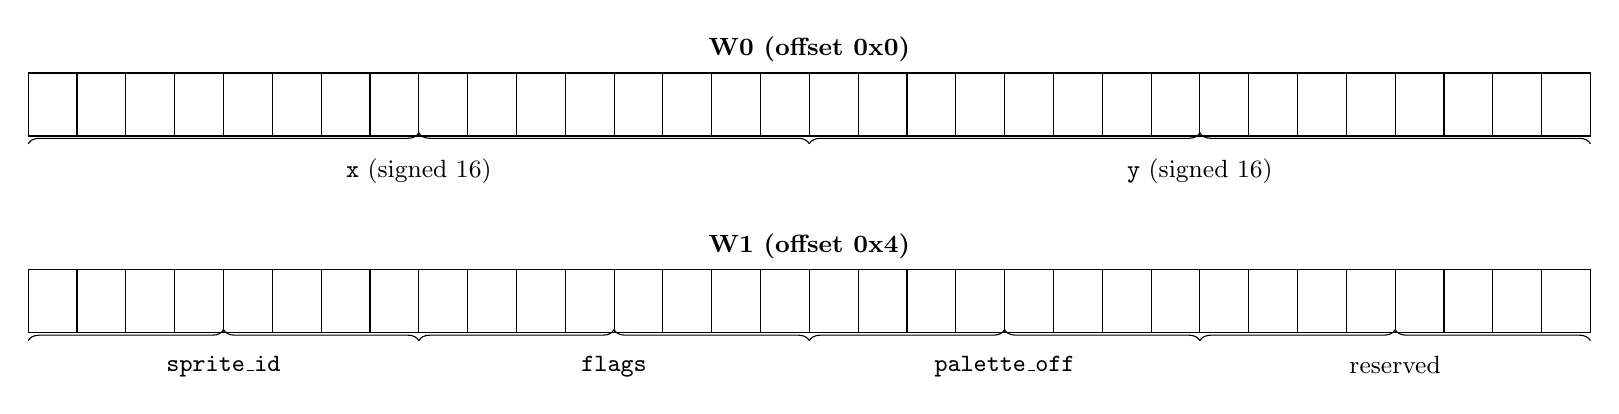
\begin{tikzpicture}[font=\small]
  \def\bw{0.62}
  \foreach \i in {0,...,31} {
    \draw (\i*\bw, 0) rectangle (\i*\bw+\bw, 0.8);
  }
  \node at (16*\bw, 1.1) {\textbf{W0 (offset 0x0)}};
  \draw[decorate,decoration={brace,amplitude=4pt}] (0, -0.1) -- (16*\bw, -0.1) node[midway,below=2pt]{\texttt{x} (signed 16)};
  \draw[decorate,decoration={brace,amplitude=4pt}] (16*\bw, -0.1) -- (32*\bw, -0.1) node[midway,below=2pt]{\texttt{y} (signed 16)};

  \begin{scope}[yshift=-2.5cm]
    \foreach \i in {0,...,31} {
      \draw (\i*\bw, 0) rectangle (\i*\bw+\bw, 0.8);
    }
    \node at (16*\bw, 1.1) {\textbf{W1 (offset 0x4)}};
    \draw[decorate,decoration={brace,amplitude=4pt}] (0, -0.1) -- (8*\bw, -0.1) node[midway,below=2pt]{\texttt{sprite\_id}};
    \draw[decorate,decoration={brace,amplitude=4pt}] (8*\bw, -0.1) -- (16*\bw, -0.1) node[midway,below=2pt]{\texttt{flags}};
    \draw[decorate,decoration={brace,amplitude=4pt}] (16*\bw, -0.1) -- (24*\bw, -0.1) node[midway,below=2pt]{\texttt{palette\_off}};
    \draw[decorate,decoration={brace,amplitude=4pt}] (24*\bw, -0.1) -- (32*\bw, -0.1) node[midway,below=2pt]{reserved};
  \end{scope}
\end{tikzpicture}}

\vspace{0.6cm}
\textbf{flags byte:} \quad
\texttt{[2]} hflip\quad
\texttt{[3]} vflip\quad
\texttt{[6:4]} priority (0 = highest)\quad
\texttt{[7]} ACTIVE
\end{frame}

% ===========================================================================
\begin{frame}{Frame commit --- shadow $\rightarrow$ active at VSYNC}
\centering
\resizebox{0.95\textwidth}{!}{%
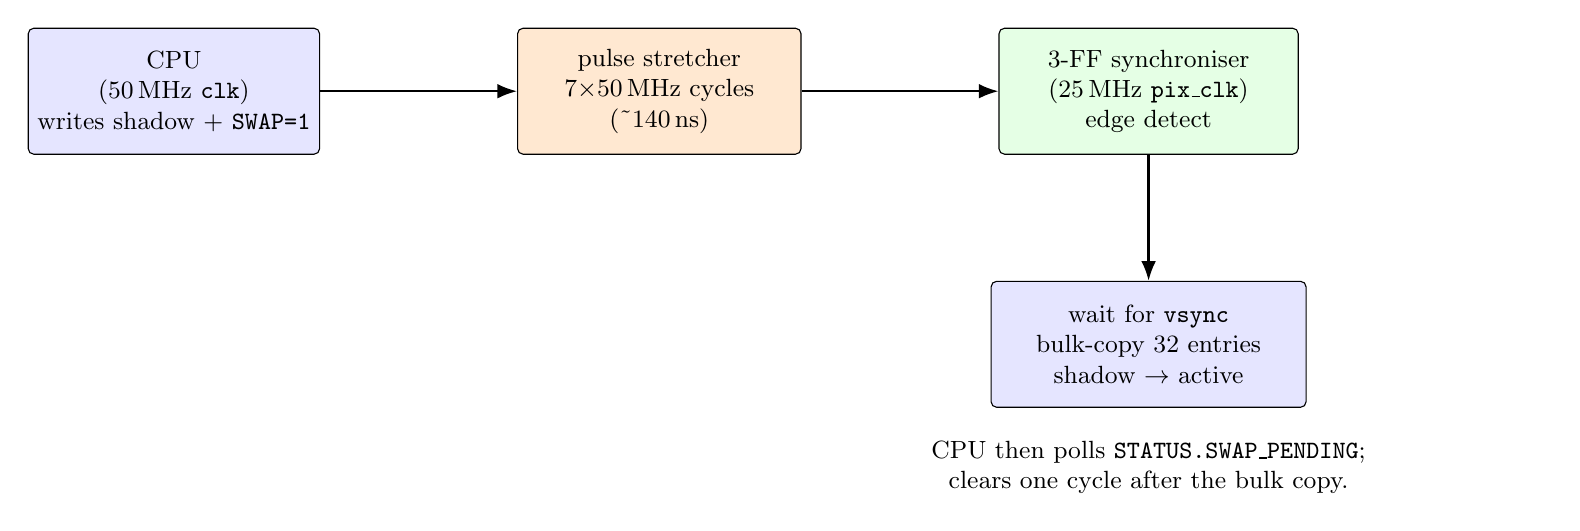
\begin{tikzpicture}[font=\small]
  \node[blk, fill=blue!10, minimum width=3.6cm, minimum height=1.6cm] (cpu) {CPU \\ (50\,MHz \texttt{clk}) \\ writes shadow + \texttt{SWAP=1}};
  \node[blk, right=2.5cm of cpu, fill=orange!18, minimum width=3.6cm, minimum height=1.6cm] (str) {pulse stretcher \\ 7$\times$50\,MHz cycles \\ (\textasciitilde 140\,ns)};
  \node[blk, right=2.5cm of str, fill=green!10, minimum width=3.8cm, minimum height=1.6cm] (sync) {3-FF synchroniser \\ (25\,MHz \texttt{pix\_clk}) \\ edge detect};
  \node[blk, below=1.6cm of sync, fill=blue!10, minimum width=4.0cm, minimum height=1.6cm] (swap) {wait for \texttt{vsync} \\ bulk-copy 32 entries \\ shadow $\to$ active};

  \draw[arr] (cpu) -- (str);
  \draw[arr] (str) -- (sync);
  \draw[arr] (sync) -- (swap);

  \node[below=0.3cm of swap, text width=10cm, align=center, font=\small]
    {CPU then polls \texttt{STATUS.SWAP\_PENDING}; clears one cycle after the bulk copy.};
\end{tikzpicture}}

\vspace{0.3cm}
\small One 20\,ns Avalon pulse would slip past the 40\,ns pixel clock. Widen to 140\,ns and the CDC is deterministic.
\end{frame}

% ===========================================================================
\begin{frame}{Tile-map byte writes --- packed \texttt{[3:0][7:0]}}
\centering
\resizebox{0.95\textwidth}{!}{%
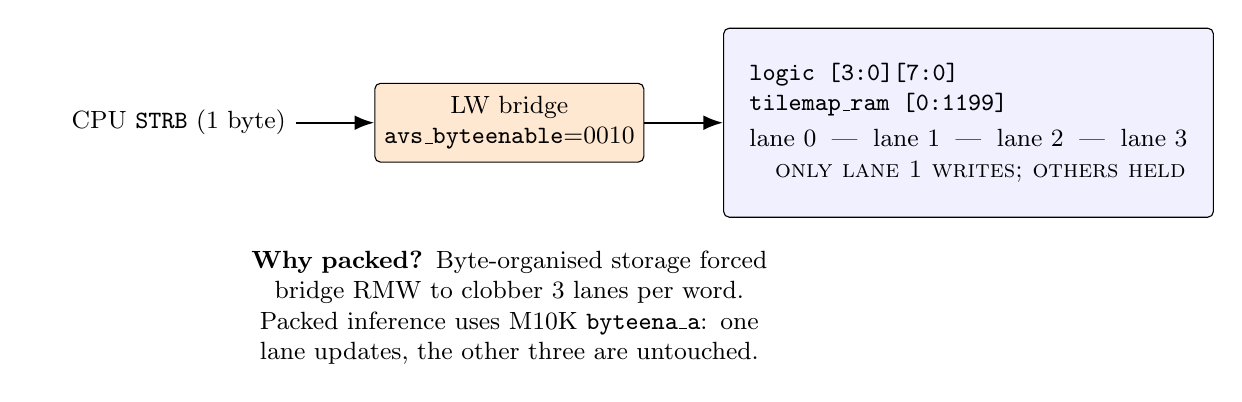
\begin{tikzpicture}[font=\small]
  \node (cpu) {CPU \texttt{STRB} (1 byte)};
  \node[blk, fill=orange!18, right=1cm of cpu, minimum width=3.4cm] (br) {LW bridge \\ \texttt{avs\_byteenable}=0010};
  \node[blk, right=1cm of br, minimum width=5.0cm, minimum height=2.4cm, fill=blue!6, align=left] (ram)
    {\begin{tabular}{l}
      \texttt{logic [3:0][7:0]} \\
      \texttt{tilemap\_ram [0:1199]} \\[2pt]
      lane 0 \;|\; lane 1 \;|\; lane 2 \;|\; lane 3 \\
      \quad\textsc{only lane 1 writes; others held}
     \end{tabular}};
  \draw[arr] (cpu) -- (br);
  \draw[arr] (br) -- (ram);

  \node[below=1.0cm of br, text width=12cm, align=center]
    {\textbf{Why packed?} Byte-organised storage forced bridge RMW to clobber 3 lanes per word.\\
     Packed inference uses M10K \texttt{byteena\_a}: one lane updates, the other three are untouched.};
\end{tikzpicture}}
\end{frame}

% ===========================================================================
\begin{frame}{VGA timing --- 640$\times$480 @ 60\,Hz, 25\,MHz dot}
\centering
\resizebox{0.7\textwidth}{!}{%
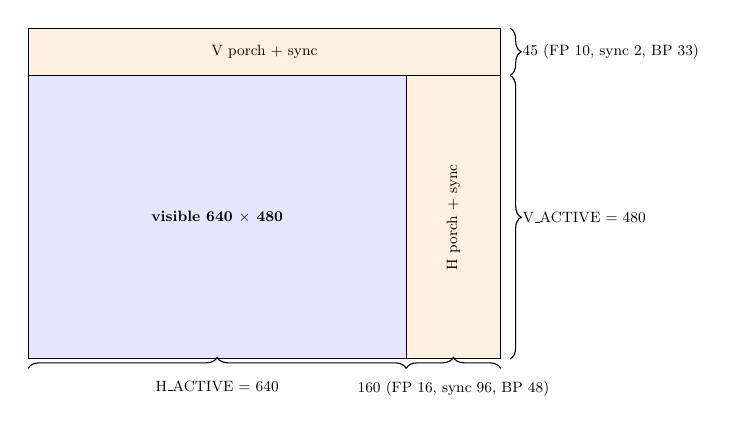
\begin{tikzpicture}[font=\small, scale=0.6, every node/.style={transform shape}]
  \draw[fill=blue!10] (0,0) rectangle (8,6);
  \node at (4,3) {\textbf{visible 640 $\times$ 480}};
  \draw[fill=orange!12] (8,0) rectangle (10,6); \node[rotate=90] at (9,3) {H porch + sync};
  \draw[fill=orange!12] (0,6) rectangle (10,7); \node at (5,6.5) {V porch + sync};

  \draw[decorate,decoration={brace,amplitude=4pt}] (0,-0.2) -- (8,-0.2) node[midway,below=4pt]{H\_ACTIVE = 640};
  \draw[decorate,decoration={brace,amplitude=4pt}] (8,-0.2) -- (10,-0.2) node[midway,below=4pt]{160 (FP 16, sync 96, BP 48)};
  \draw[decorate,decoration={brace,amplitude=4pt,mirror}] (10.2,0) -- (10.2,6) node[midway,right=4pt]{V\_ACTIVE = 480};
  \draw[decorate,decoration={brace,amplitude=4pt,mirror}] (10.2,6) -- (10.2,7) node[midway,right=4pt]{45 (FP 10, sync 2, BP 33)};
\end{tikzpicture}}

\vspace{0.2cm}
\small One frame = 800 $\times$ 525 dot cycles. HBLANK is the 160-cycle window we use to evaluate sprites for the next scanline.
\end{frame}

% ===========================================================================
\begin{frame}{Pixel pipeline --- sprite engine + compositor}
\centering
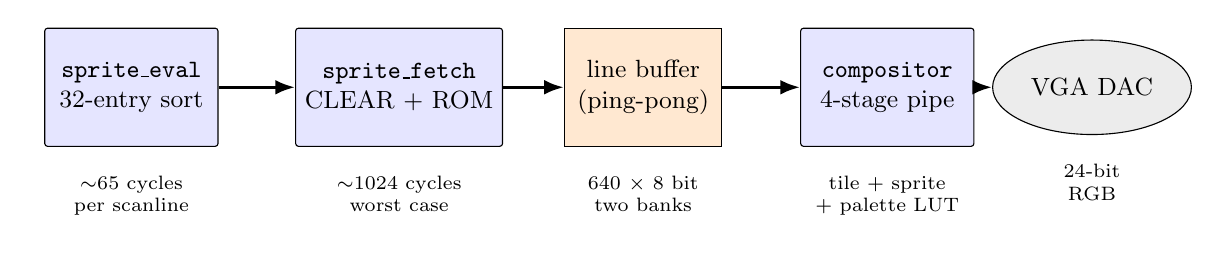
\begin{tikzpicture}[font=\footnotesize]
  % Five blocks evenly spaced. Wider gaps; no labels on arrows --
  % the under-block annotations carry the cycle/format info.
  \node[pipe, fill=blue!10, minimum width=2.2cm, minimum height=1.5cm] (eval)  at (0,0)     {\texttt{sprite\_eval}\\32-entry sort};
  \node[pipe, fill=blue!10, minimum width=2.2cm, minimum height=1.5cm] (fetch) at (3.4,0)   {\texttt{sprite\_fetch}\\CLEAR + ROM};
  \node[mem,  fill=orange!18, minimum width=2.0cm, minimum height=1.5cm] (lbuf) at (6.5,0)  {line buffer\\(ping-pong)};
  \node[pipe, fill=blue!10, minimum width=2.2cm, minimum height=1.5cm] (comp)  at (9.6,0)   {\texttt{compositor}\\4-stage pipe};
  \node[io,  minimum width=1.6cm, minimum height=1.2cm]                (rgb)  at (12.2,0)  {VGA DAC};

  \draw[arr, very thick] (eval)  -- (fetch);
  \draw[arr, very thick] (fetch) -- (lbuf);
  \draw[arr, very thick] (lbuf)  -- (comp);
  \draw[arr, very thick] (comp)  -- (rgb);

  % Cycle/data annotations BELOW each block
  \node[below=0.25cm of eval,  font=\scriptsize, align=center, text width=2.4cm]{$\sim$65 cycles\\per scanline};
  \node[below=0.25cm of fetch, font=\scriptsize, align=center, text width=2.4cm]{$\sim$1024 cycles\\worst case};
  \node[below=0.25cm of lbuf,  font=\scriptsize, align=center, text width=2.2cm]{640 $\times$ 8 bit\\two banks};
  \node[below=0.25cm of comp,  font=\scriptsize, align=center, text width=2.4cm]{tile + sprite\\+ palette LUT};
  \node[below=0.25cm of rgb,   font=\scriptsize, align=center, text width=1.8cm]{24-bit\\RGB};
\end{tikzpicture}

\vspace{0.5cm}
\small Eval runs inside HBLANK (160 cycles). Fetch spans HBLANK + visible (800 cycles).\\
Line buffers are double-buffered, so fetch lags read by one scanline. Compositor never stalls.
\end{frame}

% ===========================================================================
\begin{frame}{\texttt{sprite\_eval} --- per-scanline priority sort}
\centering
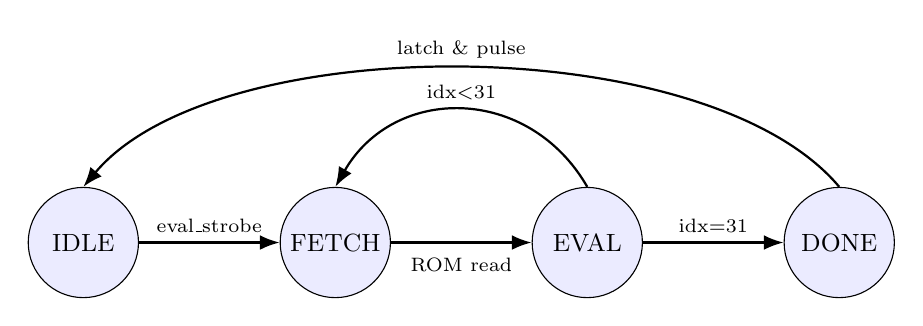
\begin{tikzpicture}[font=\small]
  \node[fsm] (idle)  at (0,0)   {IDLE};
  \node[fsm] (fetch) at (3.2,0) {FETCH};
  \node[fsm] (eval)  at (6.4,0) {EVAL};
  \node[fsm] (done)  at (9.6,0) {DONE};

  % Forward arrows on the row
  \draw[arr] (idle)  -- (fetch) node[midway, above, font=\scriptsize]{eval\_strobe};
  \draw[arr] (fetch) -- (eval)  node[midway, below=2pt, font=\scriptsize]{ROM read};
  \draw[arr] (eval)  -- (done)  node[midway, above, font=\scriptsize]{idx=31};

  % Bend-back arrows, well above the row, clearly above the labels
  \draw[arr] (eval.north) to[out=120, in=60, looseness=1.2]
       node[midway, above, font=\scriptsize]{idx$<$31} (fetch.north);
  \draw[arr] (done.north) to[out=130, in=50, looseness=0.7]
       node[midway, above, font=\scriptsize]{latch \& pulse} (idle.north);
\end{tikzpicture}

\vspace{0.8cm}
\begin{minipage}{0.85\linewidth}
\small
Per sprite (1 cycle in EVAL):\\
\quad\texttt{intersects = active \&\& y$\leq$next\_scanline $<$ y+16}\\
\quad insertion-sort into 8 priority-ordered slots (all 8 compares in parallel)\\[4pt]
Total: 32 fetch+eval cycles $+$ 1 DONE = $\sim$65 cycles.\quad Fits easily in 160-cycle HBLANK.
\end{minipage}
\end{frame}

% ===========================================================================
\begin{frame}{\texttt{sprite\_fetch} --- ROM read + line-buffer fill}
\centering
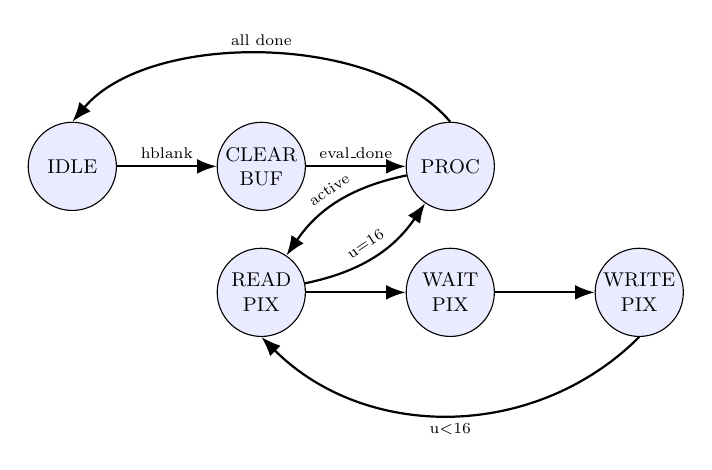
\begin{tikzpicture}[font=\footnotesize, scale=0.8, every node/.style={transform shape}]
  % Top row: control states
  \node[fsm] (idle) at (0,    1.0)  {IDLE};
  \node[fsm] (clr)  at (3,    1.0)  {CLEAR\\BUF};
  \node[fsm] (proc) at (6,    1.0)  {PROC};
  % Bottom row: per-pixel inner loop
  \node[fsm] (rd)   at (3,   -1.0)  {READ\\PIX};
  \node[fsm] (wt)   at (6,   -1.0)  {WAIT\\PIX};
  \node[fsm] (wr)   at (9,   -1.0)  {WRITE\\PIX};

  % Top-row forward edges
  \draw[arr] (idle) -- (clr)  node[midway, above, font=\scriptsize]{hblank};
  \draw[arr] (clr)  -- (proc) node[midway, above, font=\scriptsize]{eval\_done};

  % PROC down to RD (curves to upper-left of midline) ---
  \draw[arr] (proc) to[bend right=22]
       node[midway, sloped, above=1pt, font=\scriptsize]{active} (rd);

  % Bottom row forward edges
  \draw[arr] (rd) -- (wt);
  \draw[arr] (wt) -- (wr);

  % u<16: WRITE bends back to READ (arc below the bottom row)
  \draw[arr] (wr.south) to[bend left=45]
       node[midway, below, font=\scriptsize]{u$<$16} (rd.south);

  % RD up to PROC (same nodes but curves to lower-right of midline) ---
  \draw[arr] (rd) to[bend right=22]
       node[midway, sloped, above=1pt, font=\scriptsize]{u=16} (proc);

  % all done: PROC arcs above the top row back to IDLE
  \draw[arr] (proc.north) to[out=130, in=50, looseness=0.8]
       node[midway, above, font=\scriptsize]{all done} (idle.north);
\end{tikzpicture}

\smallskip
\footnotesize
\textbf{Worst-case cycle budget per scanline:}\quad
CLEAR\_BUF (640) + 8 sprites $\times$ 48 (384) $= \sim$1024 cycles.\\
HBLANK alone is 160; HBLANK + visible is \textbf{800}.\quad
Fetch lives one line behind the read, so the ping-pong line buffers absorb the latency.
\end{frame}

% ===========================================================================
\begin{frame}{Compositor --- 4-stage pipeline}
\centering
\resizebox{0.95\textwidth}{!}{%
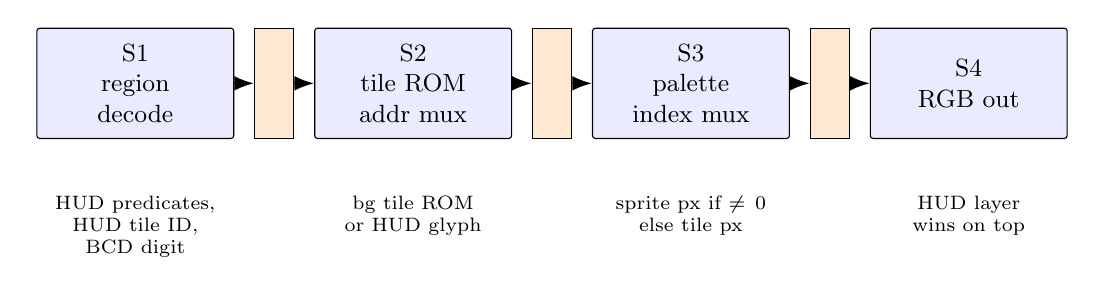
\begin{tikzpicture}[font=\small]
  \node[pipe] (s1) {S1\\region\\decode};
  \node[latch, right=0.25cm of s1] (l1) {};
  \node[pipe, right=0.25cm of l1] (s2) {S2\\tile ROM\\addr mux};
  \node[latch, right=0.25cm of s2] (l2) {};
  \node[pipe, right=0.25cm of l2] (s3) {S3\\palette\\index mux};
  \node[latch, right=0.25cm of s3] (l3) {};
  \node[pipe, right=0.25cm of l3] (s4) {S4\\RGB out};

  \draw[arr] (s1) -- (l1); \draw[arr] (l1) -- (s2);
  \draw[arr] (s2) -- (l2); \draw[arr] (l2) -- (s3);
  \draw[arr] (s3) -- (l3); \draw[arr] (l3) -- (s4);

  \node[below=0.6cm of s1, font=\scriptsize, align=center, text width=2.5cm]
    {HUD predicates,\\HUD tile ID,\\BCD digit};
  \node[below=0.6cm of s2, font=\scriptsize, align=center, text width=2.5cm]
    {bg tile ROM\\or HUD glyph};
  \node[below=0.6cm of s3, font=\scriptsize, align=center, text width=2.5cm]
    {sprite px if $\neq 0$\\else tile px};
  \node[below=0.6cm of s4, font=\scriptsize, align=center, text width=2.5cm]
    {HUD layer\\wins on top};
\end{tikzpicture}}

\vspace{0.4cm}
\small Latches between stages absorb the 1-cycle latency of tile ROM and palette M10K reads. Never stalls.
\end{frame}

% ===========================================================================
\begin{frame}{HUD strip --- top 16 pixels of every frame}
\centering
\resizebox{0.95\textwidth}{!}{%
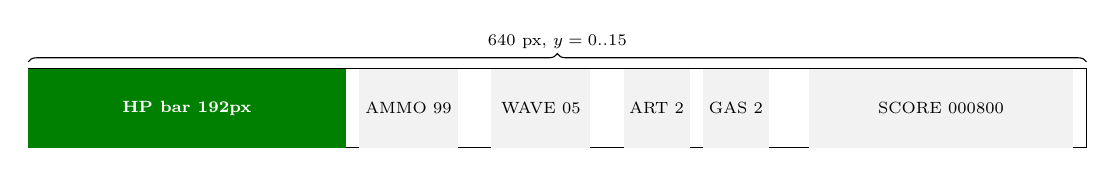
\begin{tikzpicture}[font=\scriptsize, scale=0.84, every node/.style={transform shape}]
  \draw[draw=black] (0,0) rectangle (16,1.2);
  \fill[green!50!black]    (0,0)   rectangle (4.8,1.2); \node[white] at (2.4,0.6) {\textbf{HP bar 192px}};
  \fill[gray!10] (5,0) rectangle (6.5,1.2); \node at (5.75,0.6) {AMMO 99};
  \fill[gray!10] (7,0) rectangle (8.5,1.2); \node at (7.75,0.6) {WAVE 05};
  \fill[gray!10] (9,0) rectangle (10,1.2); \node at (9.5,0.6) {ART 2};
  \fill[gray!10] (10.2,0) rectangle (11.2,1.2); \node at (10.7,0.6) {GAS 2};
  \fill[gray!10] (11.8,0) rectangle (15.8,1.2); \node at (13.8,0.6) {SCORE 000800};

  \draw[decorate,decoration={brace,amplitude=3pt}] (0,1.3) -- (16,1.3) node[midway, above=2pt]{640 px, $y=0..15$};
\end{tikzpicture}}

\vspace{0.6cm}
\small
HP bar: 2 px per HP, clamped to 192.\quad
Glyphs: 8$\times$8 from tile ROM, slots 16--41 (A--Z), 48--57 (0--9).\quad
Scores, ammo, wave packed BCD in registers.
\end{frame}

% ===========================================================================
\begin{frame}[plain]{HUD --- on the monitor}
\centering
\IfFileExists{../submission/img/02_hud_closeup.jpg}{%
  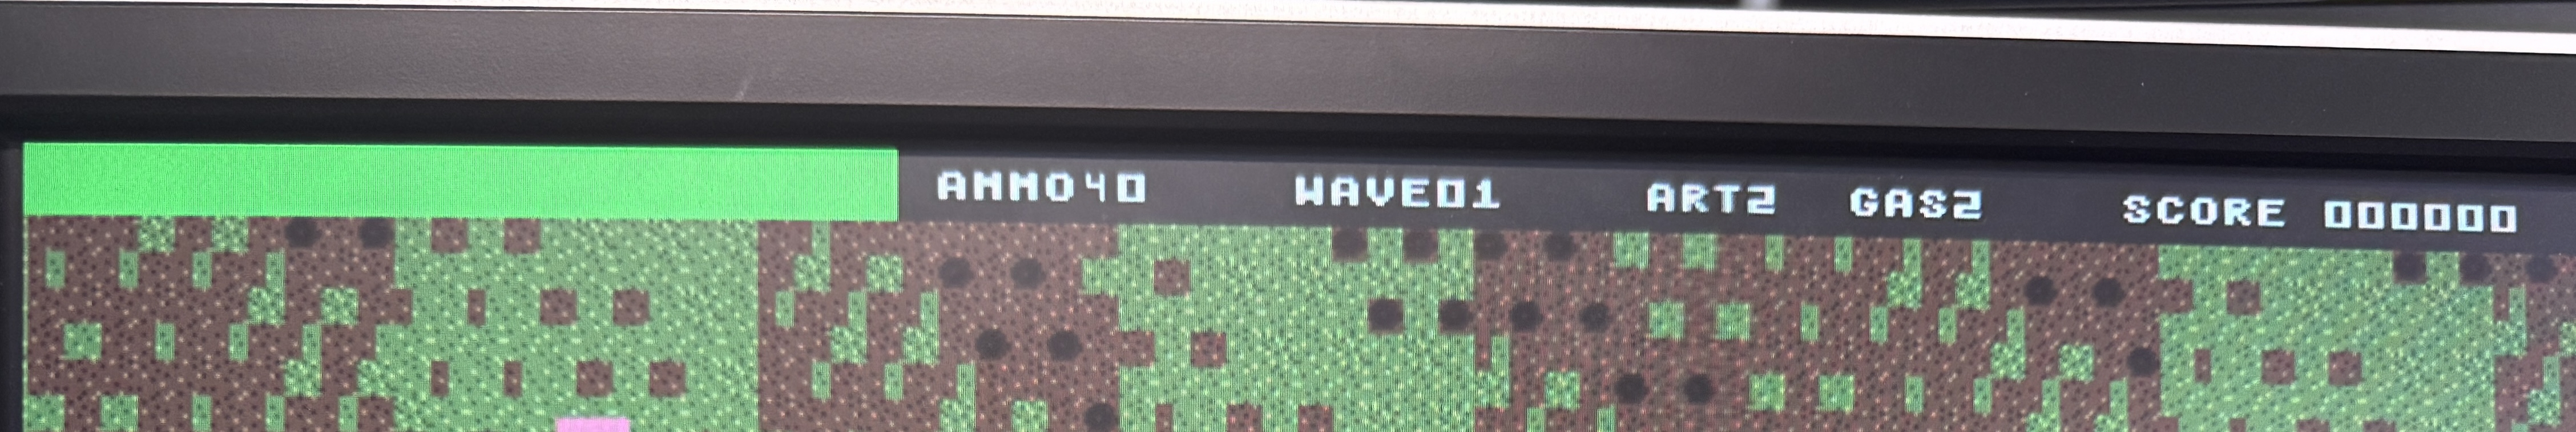
\includegraphics[width=\textwidth,height=0.85\textheight,keepaspectratio]{../submission/img/02_hud_closeup.jpg}%
}{%
  \begin{tikzpicture}
    \draw[thick,dashed,gray] (0,0) rectangle (15,7.5);
    \node at (7.5,4.2) {\Large PHOTO GOES HERE};
    \node at (7.5,3.5) {\small \texttt{submission/img/02\_hud\_closeup.jpg}};
    \node at (7.5,2.8) {\small Closeup of the HUD strip on the VGA monitor};
  \end{tikzpicture}%
}
\end{frame}

% ===========================================================================
\begin{frame}{Memory inventory (all inferred M10K)}
\centering
\small
\renewcommand{\arraystretch}{1.18}
\begin{tabular}{lll r}
\toprule
\textbf{Memory} & \textbf{Shape} & \textbf{Init} & \textbf{Bits} \\
\midrule
sprite ROM        & 16{,}384 $\times$ 8    & \texttt{\$readmemh} & 131{,}072 \\
tile ROM          & 4{,}096 $\times$ 8     & \texttt{\$readmemh} & 32{,}768 \\
tile map          & 1{,}200 $\times$ 32 (packed 4 $\times$ 8) & blank (HPS writes) & 38{,}400 \\
palette           & 256 $\times$ 24        & \texttt{\$readmemh} + HPS overrides & 6{,}144 \\
sprite table act. & 32 $\times$ 64         & via VSYNC bulk copy & 2{,}048 \\
sprite table shd. & 32 $\times$ 64         & HPS writes          & 2{,}048 \\
line buffer A     & 640 $\times$ 8         & cleared per HBLANK  & 5{,}120 \\
line buffer B     & 640 $\times$ 8         & cleared per HBLANK  & 5{,}120 \\
\midrule
\textbf{Total} & & & \textbf{86{,}144 bits} \\
\bottomrule
\end{tabular}

\vspace{0.4cm}
\small 14 M10K blocks out of 397.
\end{frame}

% ===========================================================================
\begin{frame}{Resource utilisation --- Cyclone V 5CSEMA5F31C6}
\centering
\small
\renewcommand{\arraystretch}{1.18}
\begin{tabular}{lrrr}
\toprule
\textbf{Resource} & \textbf{Used} & \textbf{Available} & \textbf{\%} \\
\midrule
ALMs              & 205    & 32{,}070    & $<\,1\%$ \\
Registers         & 365    & ---         & --- \\
Pins              & 54     & 457         & 12\% \\
Block memory bits & 86{,}144 & 4{,}065{,}280 & 2\% \\
M10K blocks       & 14     & 397         & 4\% \\
DSP blocks        & 0      & 87          & 0\% \\
\bottomrule
\end{tabular}

\vspace{0.5cm}
\small Compile time: 63\,s wall clock (Analysis 13\,s, Fitter 30\,s, Asm 12\,s, STA 8\,s).
\end{frame}

% ===========================================================================
\begin{frame}{Software architecture --- 60\,Hz game loop on the ARM}
\centering
\resizebox{0.95\textwidth}{!}{%
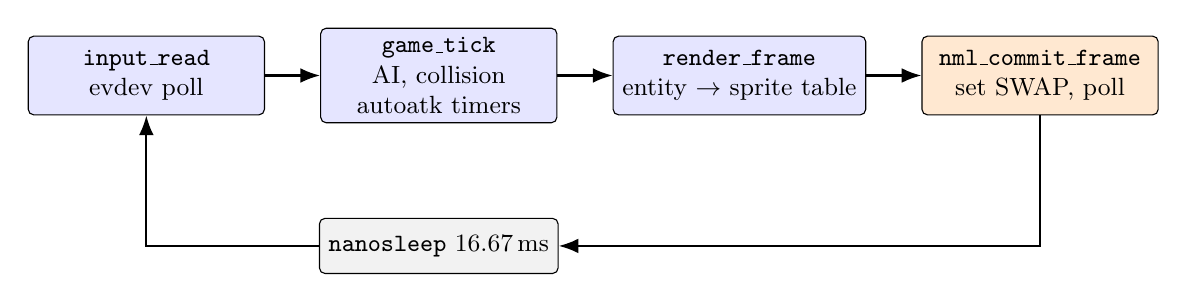
\begin{tikzpicture}[font=\small, node distance=0.7cm]
  \node[blk, fill=blue!10, minimum width=3.0cm, minimum height=1.0cm] (in)  {\texttt{input\_read}\\evdev poll};
  \node[blk, fill=blue!10, right=of in,  minimum width=3.0cm, minimum height=1.0cm] (tick){\texttt{game\_tick}\\AI, collision\\autoatk timers};
  \node[blk, fill=blue!10, right=of tick,minimum width=3.0cm, minimum height=1.0cm] (rndr){\texttt{render\_frame}\\entity $\to$ sprite table};
  \node[blk, fill=orange!18, right=of rndr, minimum width=3.0cm, minimum height=1.0cm] (cmt){\texttt{nml\_commit\_}\texttt{frame}\\set SWAP, poll};
  \node[blk, fill=gray!10, below=1.2cm of tick, minimum width=3.0cm, minimum height=0.7cm] (sleep) {\texttt{nanosleep} 16.67\,ms};

  \draw[arr] (in) -- (tick);
  \draw[arr] (tick) -- (rndr);
  \draw[arr] (rndr) -- (cmt);
  \draw[arr] (cmt.south) |- (sleep.east);
  \draw[arr] (sleep.west) -| (in.south);
\end{tikzpicture}}

\vspace{0.4cm}
\small \texttt{game\_t} holds a 64-entity pool. State machine: PLAYING $\leftrightarrow$ LEVELUP $\to$ GAMEOVER.
Mortar is timer-driven; artillery + gas fire from L/R shoulders.
\end{frame}

% ===========================================================================
\begin{frame}[plain]{What actually works}
\centering
\IfFileExists{../submission/img/03_gameplay.jpg}{%
  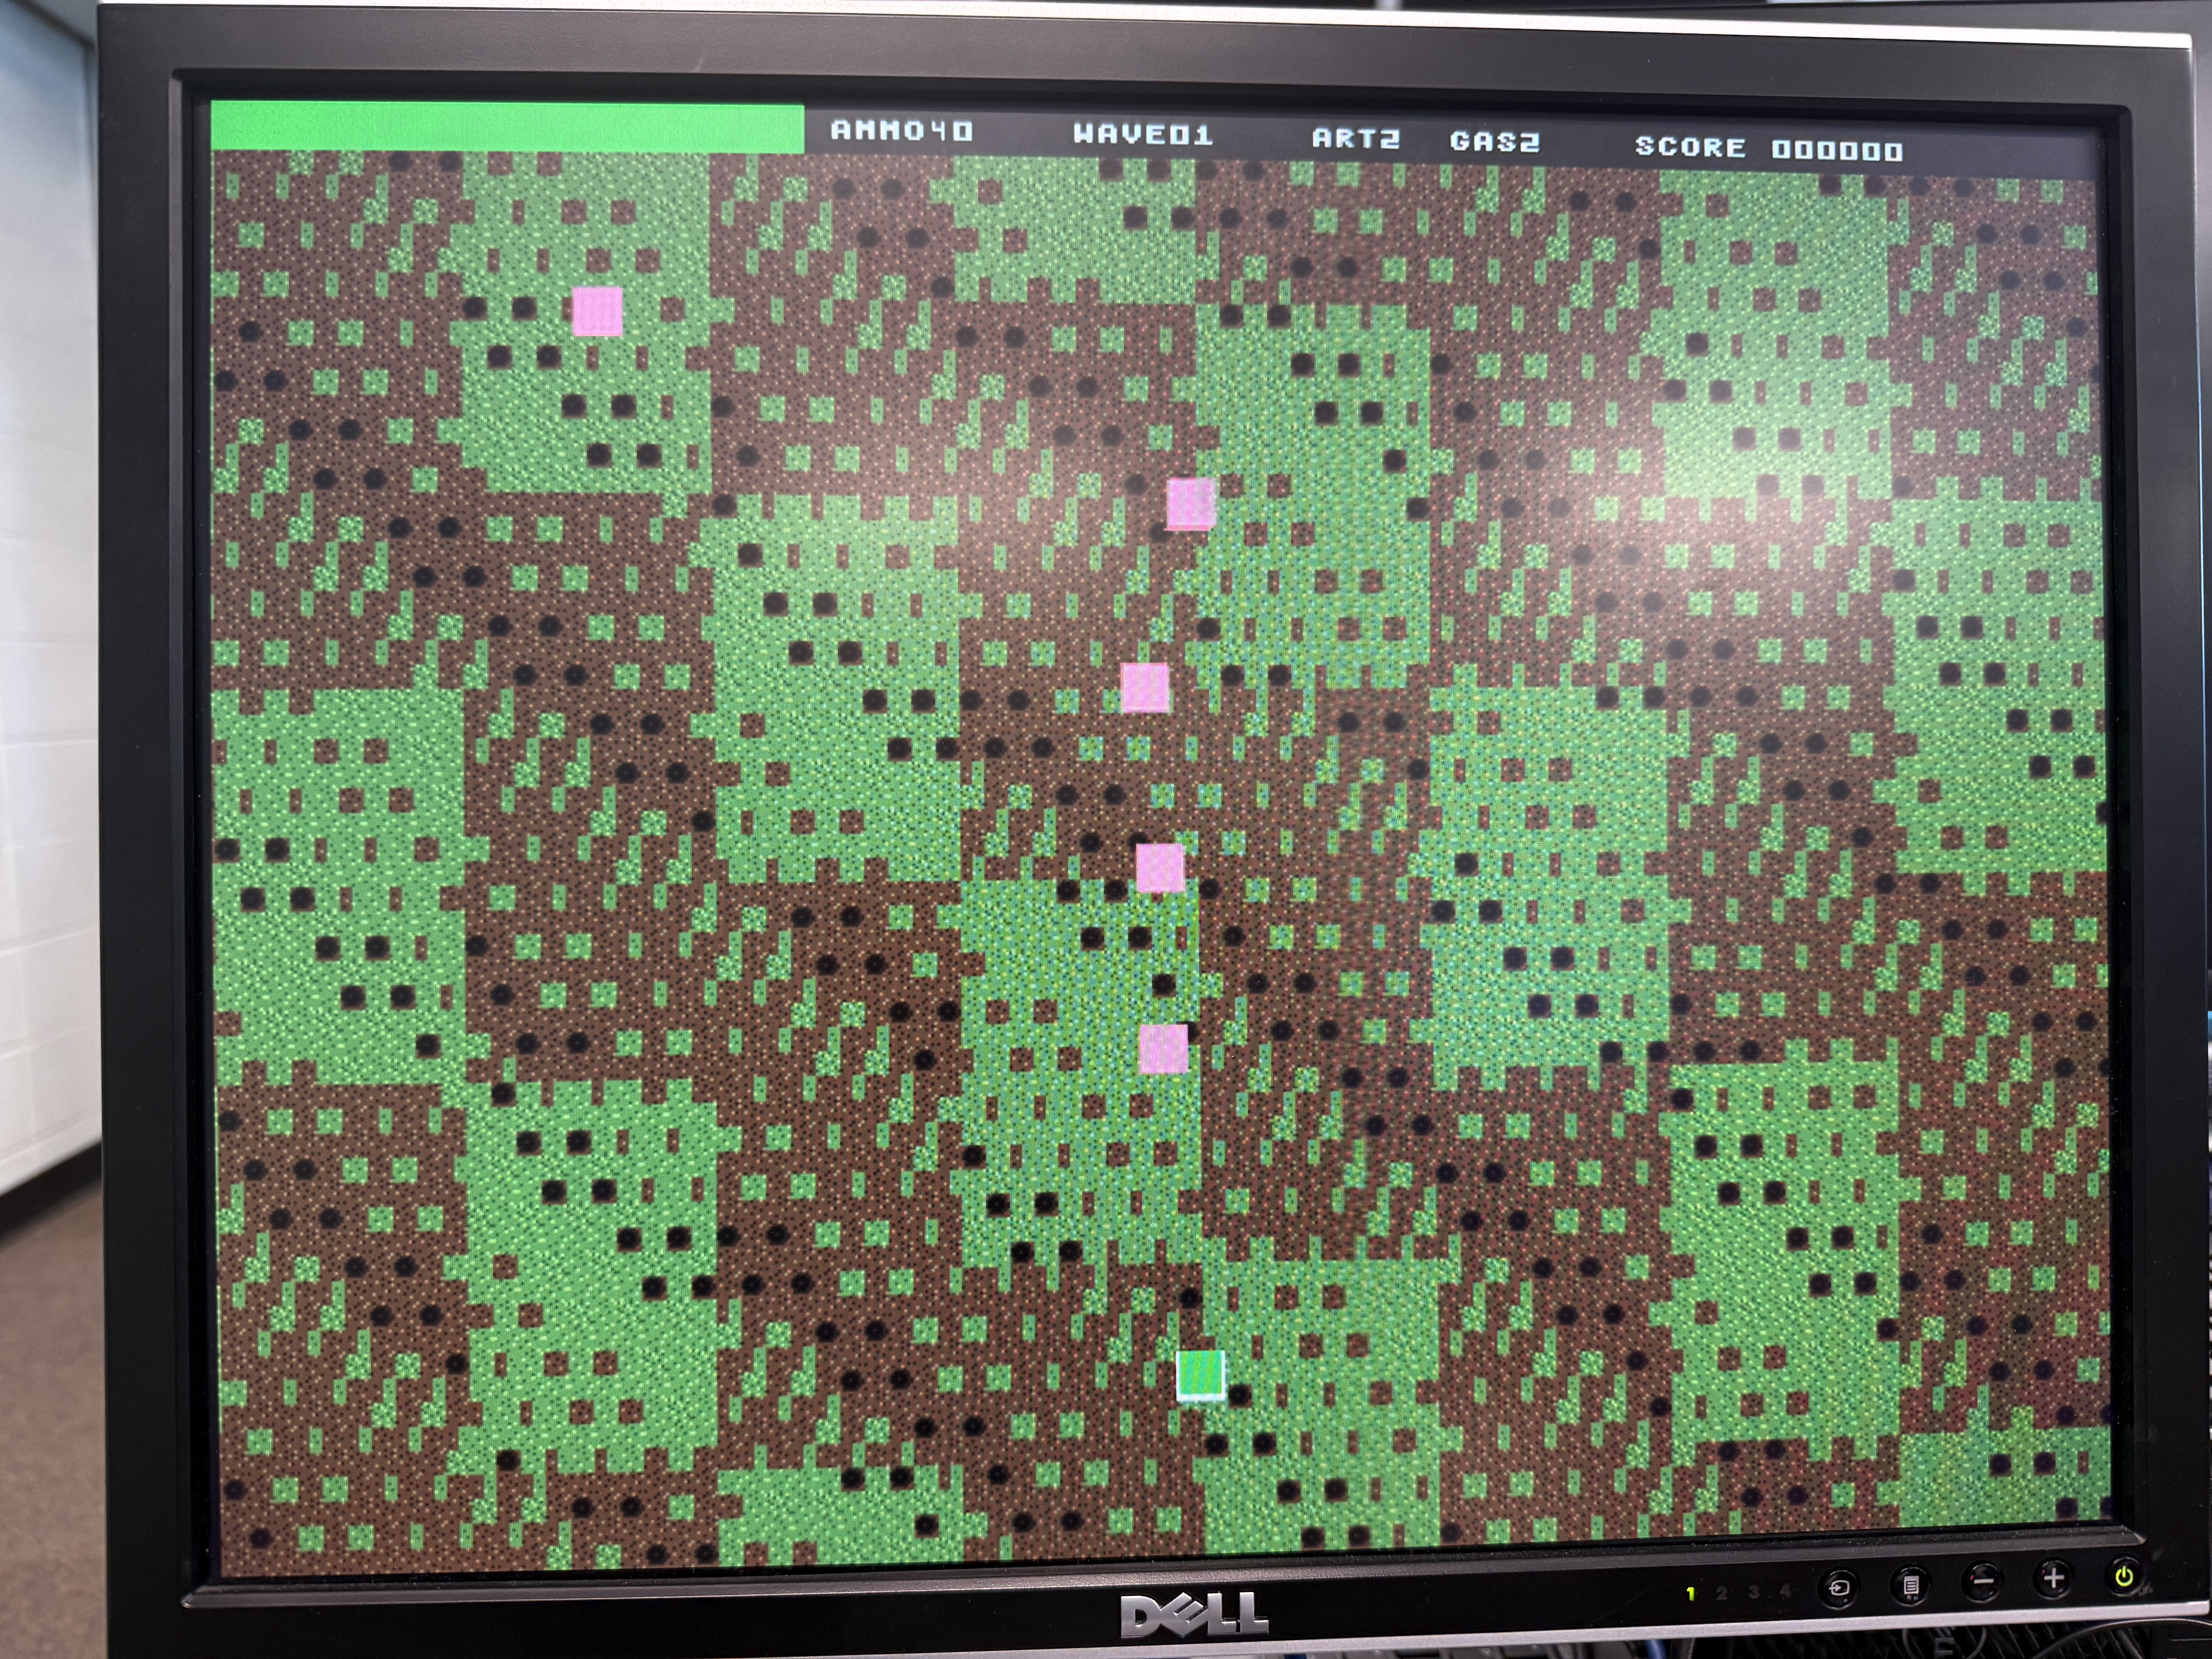
\includegraphics[width=0.92\textwidth,height=0.62\textheight,keepaspectratio]{../submission/img/03_gameplay.jpg}%
}{%
  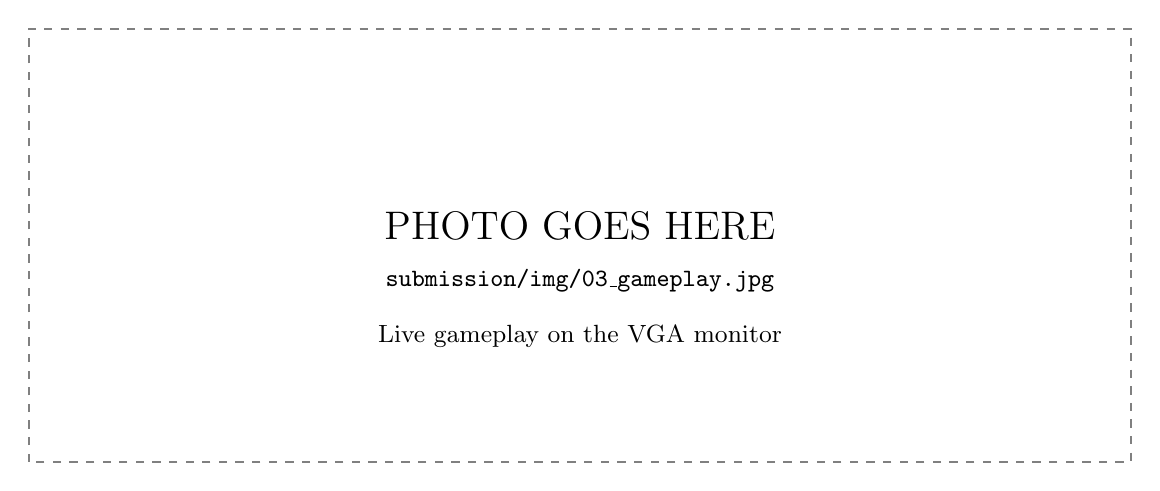
\begin{tikzpicture}
    \draw[thick,dashed,gray] (0,0) rectangle (14,5.5);
    \node at (7,3.0) {\Large PHOTO GOES HERE};
    \node at (7,2.3) {\small \texttt{submission/img/03\_gameplay.jpg}};
    \node at (7,1.6) {\small Live gameplay on the VGA monitor};
  \end{tikzpicture}%
}

\vspace{0.35cm}
\small
640$\times$480 @ 60\,Hz $\bullet$ tile-mapped battlefield $\bullet$ 32 hardware sprites $\bullet$ 256-entry palette\\
HUD: HP bar, AMMO, WAVE, ART, GAS, SCORE (BCD)\\
SNES gamepad via evdev; 60\,Hz HPS game loop; frame-commit at VSYNC\\
Mortar, artillery, gas clouds, wave spawner, level-up, ammo drops, game-over
\end{frame}

\end{document}
